%=========================================================
% Archivo:
% capitulos/04_arquitectura.tex
%=========================================================

\chapter{Arquitectura General del Sistema}

El proyecto \texttt{PDC\_FINAL} fue diseñado siguiendo una arquitectura modular que permite reutilizar el mismo algoritmo de optimización sobre diferentes paradigmas de computación paralela y distribuida. Todas las implementaciones desarrolladas comparten exactamente la misma lógica de negocio, diferenciándose únicamente en la forma en que distribuyen la carga computacional.

La arquitectura separa claramente la preparación de los datos, la ejecución del algoritmo y el registro de resultados, favoreciendo la mantenibilidad, la escalabilidad y la reproducibilidad de los experimentos.

%=========================================================
\section{Arquitectura General}

La Figura \ref{fig:arquitectura_general} presenta la organización general del sistema.

\begin{figure}[H]
    \centering
    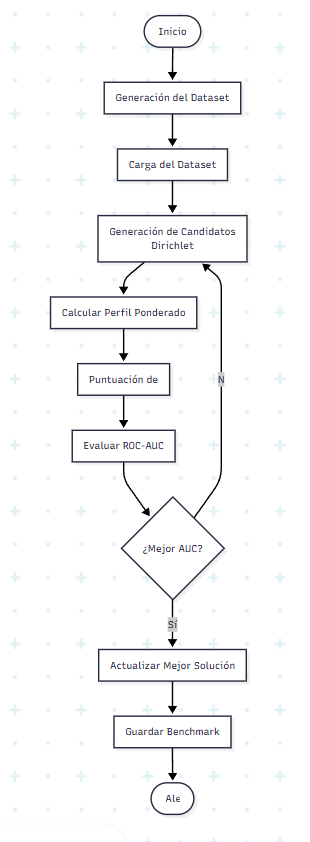
\includegraphics[width=0.95\textwidth, height=0.45\textheight, keepaspectratio]
    {figuras/arquitectura/01_arquitectura_general.png}
    \caption{Arquitectura general del sistema.}
    \label{fig:arquitectura_general}
\end{figure}

La arquitectura está compuesta por tres bloques funcionales principales:

\begin{itemize}

\item Preparación de los datos de entrada.

\item Ejecución del algoritmo de optimización.

\item Registro de métricas y resultados experimentales.

\end{itemize}

Cada bloque mantiene responsabilidades claramente definidas, permitiendo modificar una implementación sin afectar el resto del sistema.

%=========================================================
\section{Descripción del Flujo}

El proceso completo de ejecución se desarrolla mediante las siguientes etapas.

\subsection{Generación del Dataset}

Se generan o cargan los datos experimentales que servirán como entrada para el algoritmo de optimización. Dependiendo del escenario experimental, el conjunto de datos puede obtenerse desde archivos previamente construidos o mediante generación sintética.

\subsection{Carga del Dataset}

Los datos son cargados utilizando estructuras compatibles con NumPy, permitiendo realizar operaciones vectorizadas y reduciendo significativamente los tiempos de acceso durante la ejecución.

\subsection{Generación de Candidatos}

El algoritmo genera múltiples vectores de pesos utilizando una distribución de Dirichlet, garantizando que cada candidato cumpla las restricciones del simplex.

\[
\sum_{i=1}^{n} w_i = 1
\]

con

\[
w_i \geq 0
\]

Cada vector representa una posible solución al problema de optimización.

\subsection{Evaluación}

Cada candidato es evaluado mediante las siguientes operaciones:

\begin{enumerate}

\item Construcción del perfil ponderado.

\item Cálculo del \textit{Score}.

\item Evaluación de la métrica ROC-AUC.

\end{enumerate}

Dado que cada candidato puede evaluarse independientemente, esta etapa constituye el principal punto de paralelización del algoritmo.

\subsection{Selección de la Mejor Solución}

Después de evaluar todos los candidatos, el sistema conserva únicamente el vector de pesos que obtiene el mayor valor de ROC-AUC.

\subsection{Registro Experimental}

Finalmente se almacenan todas las métricas necesarias para el análisis posterior:

\begin{itemize}

\item Tiempo total de ejecución.

\item Mejor valor de ROC-AUC.

\item Vector de pesos óptimo.

\item Número de candidatos evaluados.

\item Información del entorno de ejecución.

\end{itemize}

%=========================================================
\section{Pipeline General del Proyecto}

La Figura \ref{fig:pipeline_general} resume el flujo completo seguido durante la ejecución del sistema.

\begin{figure}[H]
    \centering
    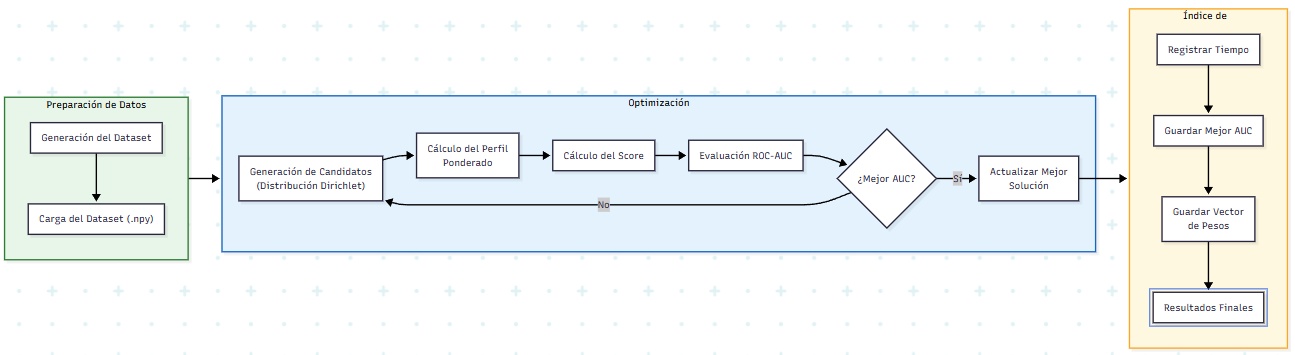
\includegraphics[width=\textwidth, height=0.45\textheight, keepaspectratio]
    {figuras/arquitectura/02_pipeline_general.png}
    \caption{Pipeline general del proyecto.}
    \label{fig:pipeline_general}
\end{figure}

El pipeline garantiza que todas las implementaciones desarrolladas ejecuten exactamente las mismas etapas del algoritmo. La única diferencia entre ellas corresponde a la estrategia utilizada para distribuir el procesamiento entre los recursos computacionales disponibles.

%=========================================================
\section{Diagrama de Componentes}

La Figura \ref{fig:componentes} presenta la organización lógica de los principales componentes software que conforman el proyecto.

\begin{figure}[H]
    \centering
    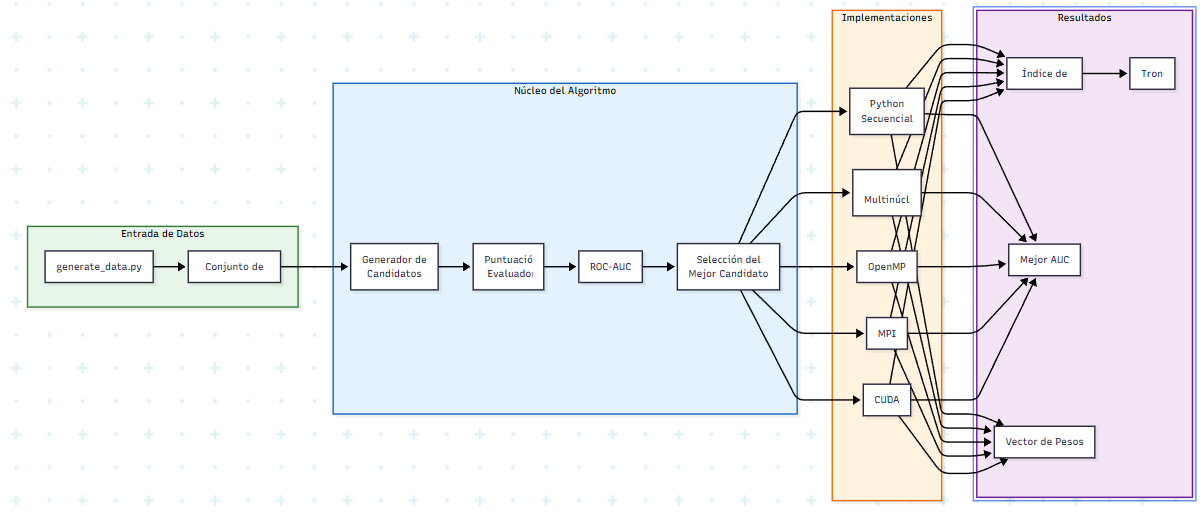
\includegraphics[width=\textwidth, height=0.45\textheight, keepaspectratio]
    {figuras/arquitectura/03_diagrama_componentes.png}
    \caption{Diagrama de componentes del sistema.}
    \label{fig:componentes}
\end{figure}

El sistema se encuentra dividido en cuatro módulos principales:

\begin{itemize}

\item Módulo de preparación y carga de datos.

\item Núcleo del algoritmo de optimización.

\item Implementaciones paralelas (Python, Multicore, OpenMP, MPI y CUDA).

\item Módulo de almacenamiento de resultados y benchmarking.

\end{itemize}

Esta organización reduce el acoplamiento entre componentes y facilita la incorporación de nuevas implementaciones sin modificar el núcleo del algoritmo.

%=========================================================
\section{Diagrama de Secuencia}

La Figura \ref{fig:secuencia} representa la interacción entre los principales componentes del sistema durante una ejecución completa del algoritmo de optimización.

\begin{figure}[H]
    \centering
    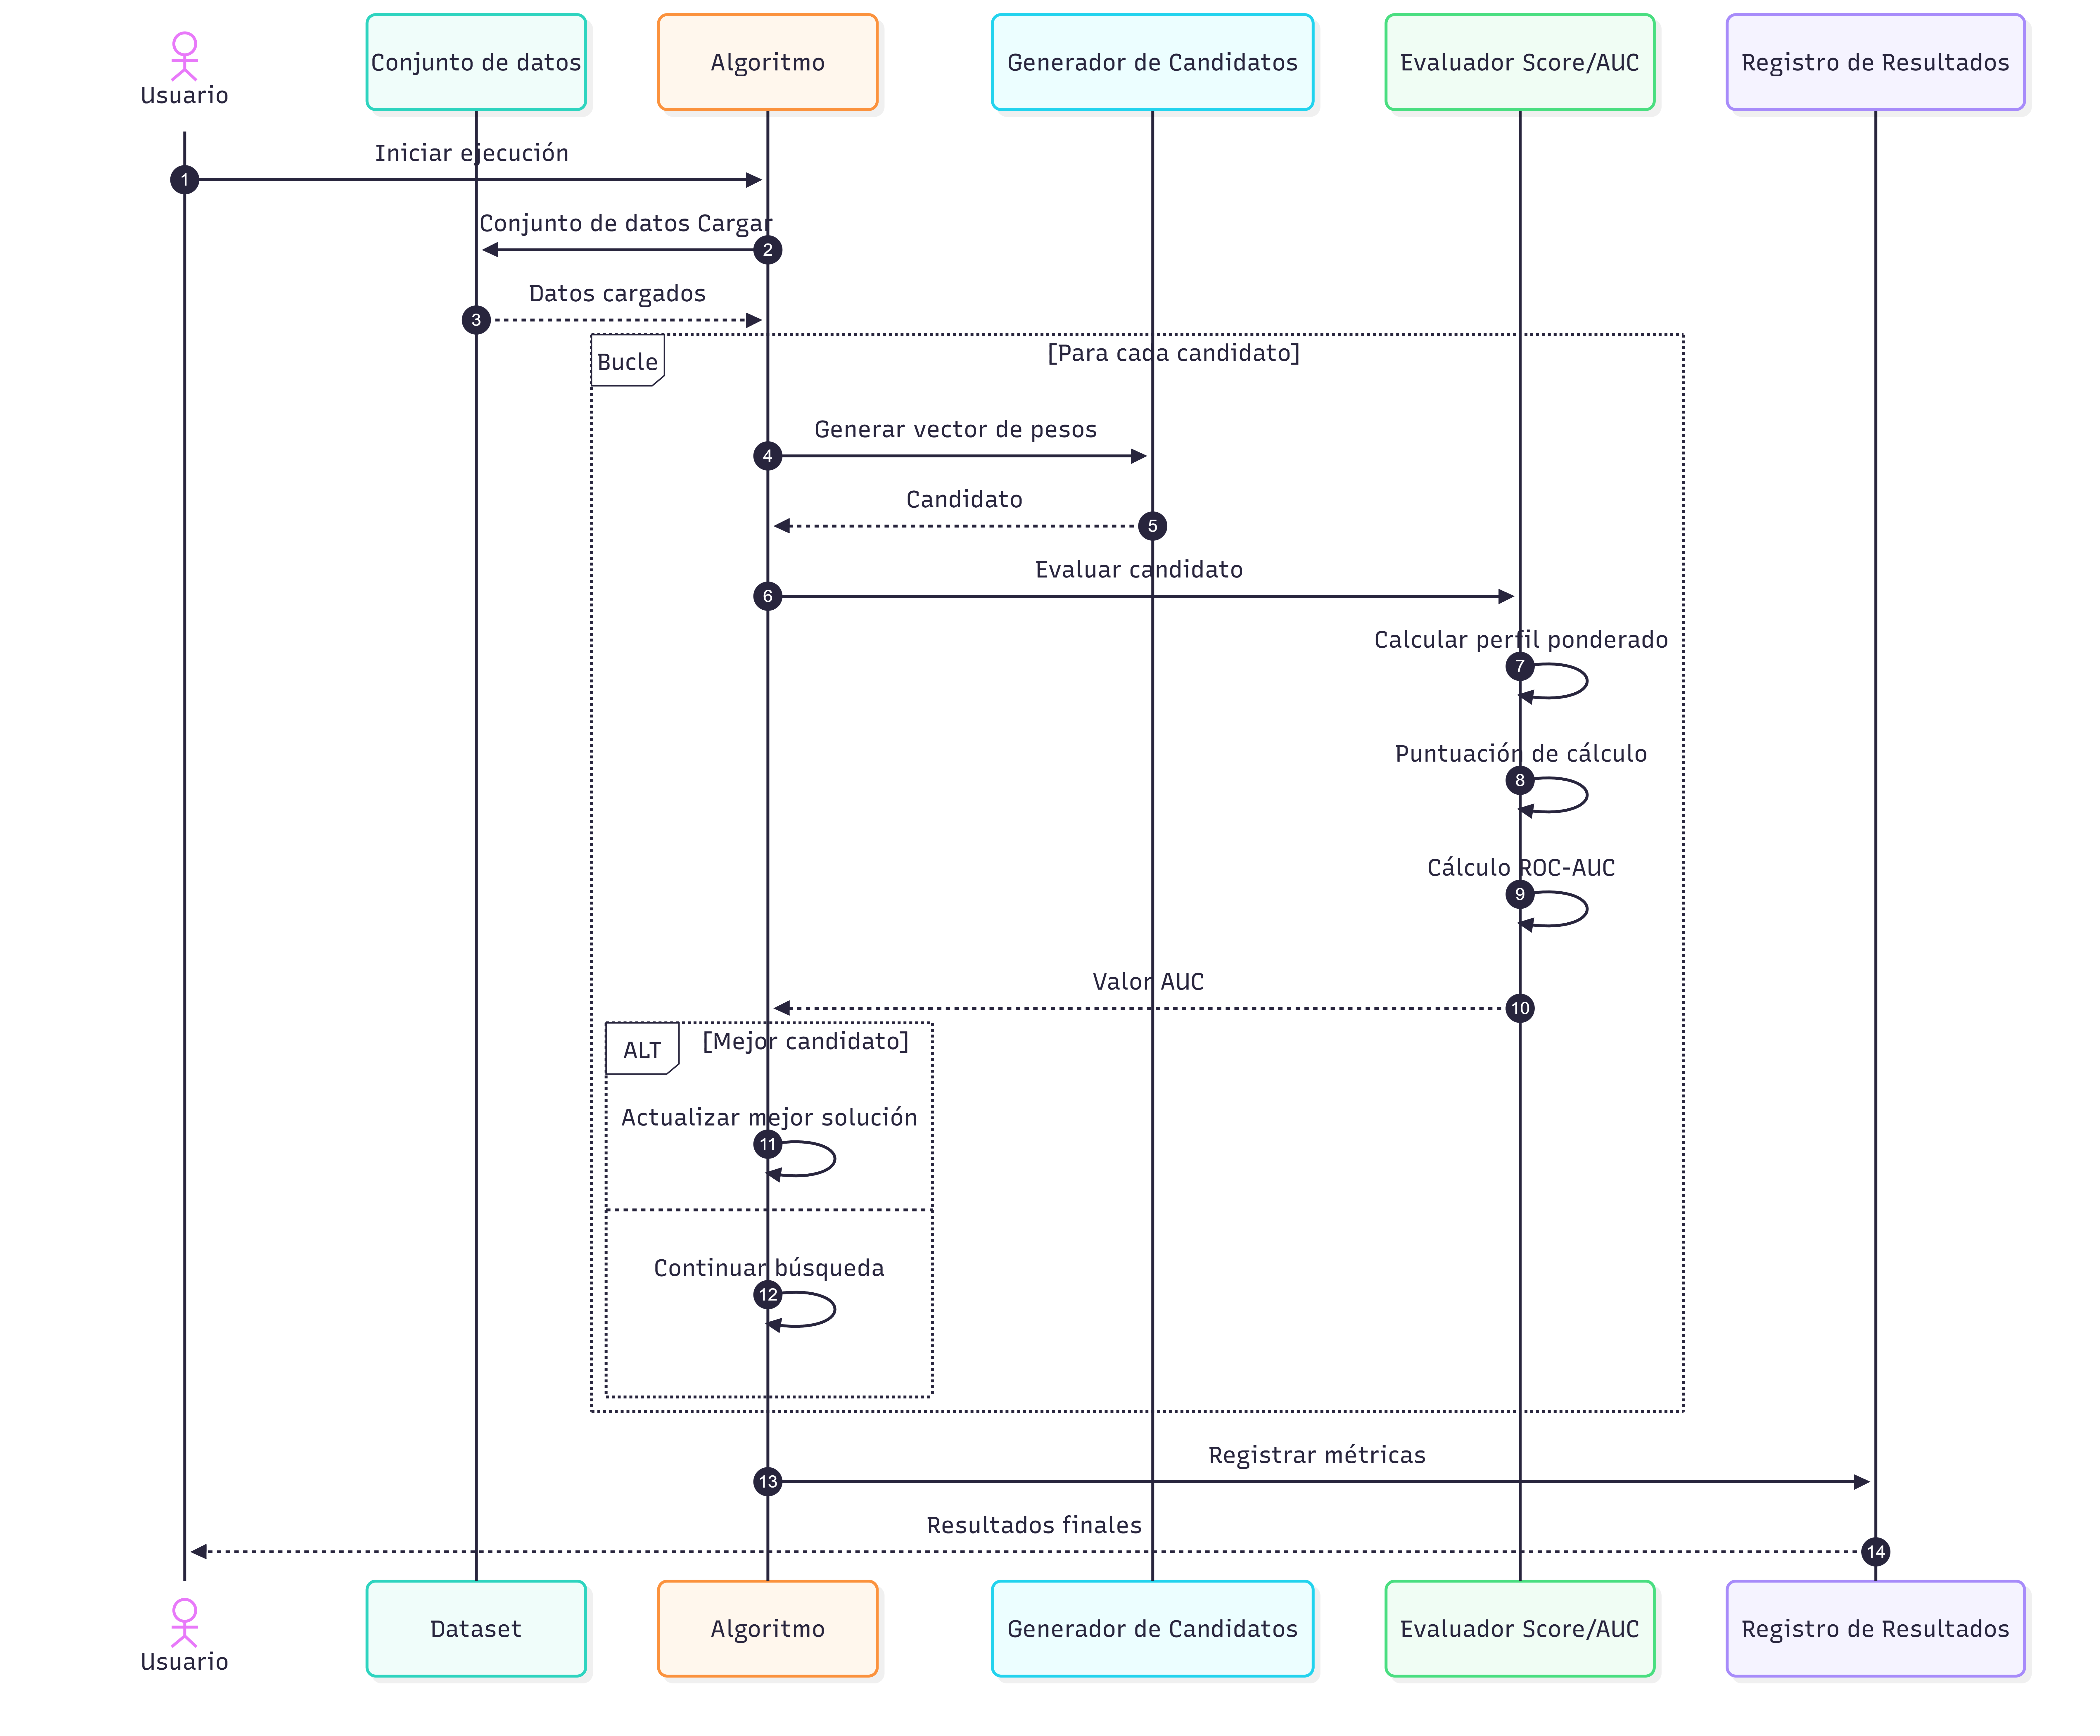
\includegraphics[width=\textwidth, height=0.45\textheight, keepaspectratio]
    {figuras/arquitectura/04_diagrama_secuencia.png}
    \caption{Diagrama de secuencia del proceso de optimización.}
    \label{fig:secuencia}
\end{figure}

El proceso inicia con la solicitud de ejecución por parte del usuario, seguida de la carga del conjunto de datos. Posteriormente, el sistema genera múltiples candidatos que son evaluados de forma independiente mediante el cálculo del perfil ponderado, el \textit{Score} y la métrica ROC-AUC. Finalmente, el mejor candidato encontrado es almacenado junto con las métricas experimentales obtenidas.

%=========================================================
\section{Características de la Arquitectura}

La arquitectura propuesta presenta las siguientes características:

\begin{itemize}

\item Modularidad.

\item Bajo acoplamiento entre componentes.

\item Alta cohesión funcional.

\item Separación entre la lógica del algoritmo y la estrategia de paralelización.

\item Reutilización del núcleo del algoritmo.

\item Escalabilidad para incorporar nuevas tecnologías.

\item Facilidad para realizar experimentos reproducibles.

\item Comparación objetiva entre las distintas implementaciones.

\end{itemize}

%=========================================================
\section{Ventajas del Diseño}

El diseño arquitectónico adoptado permitió implementar cinco versiones del mismo algoritmo utilizando diferentes paradigmas de computación de alto desempeño sin modificar su funcionamiento interno.

La reutilización del núcleo del algoritmo garantiza que todas las implementaciones trabajen sobre el mismo conjunto de datos, ejecuten exactamente la misma lógica de optimización y utilicen los mismos criterios de evaluación.

Como consecuencia, las diferencias observadas durante los experimentos corresponden exclusivamente a la estrategia de paralelización empleada y no a modificaciones en el algoritmo, permitiendo realizar comparaciones objetivas entre las versiones secuencial, multicore, OpenMP, MPI y CUDA.

Finalmente, la arquitectura modular facilita el mantenimiento del proyecto y proporciona una base sólida para incorporar futuras implementaciones o nuevas estrategias de optimización sin afectar el resto del sistema.